\documentclass[12pt,a4paper,titlepage]{article}

\usepackage[ngerman]{babel}
\usepackage[utf8x]{inputenc}
\usepackage{graphicx}
\usepackage[printonlyused,withpage]{acronym}
\usepackage{tocstyle}
\usepackage{harvard}
\usepackage{tocloft}
\usepackage{amsmath}
\usepackage{framed}

\newcommand{\listequationsname}{\Large{Formelverzeichnis}} 
\newlistof{myequations}{equ}{\listequationsname} 
\newcommand{\myequations}[1]{% 
\addcontentsline{equ}{myequations}{\protect\numberline{\theequation}#1}\par} 

\title{
\includegraphics[scale=0.3]{img/logo_htw}\\~\\~\\
Positionierung in Sensornetzen}
\author{Andr\'{e} Vogler \& Torsten Braun}
\date{\today}

\begin{document}
\pagenumbering{Roman} 
\maketitle
\tableofcontents
\newpage
\addcontentsline{toc}{section}{Abbildungsverzeichnis}
\listoffigures
\newpage
\addcontentsline{toc}{section}{Formelverzeichnis}
\listofmyequations
\section*{Abkürzungsverzeichnis}
\addcontentsline{toc}{section}{Abkürzungsverezichnis}

\begin{acronym}[RSSI]
  \acro{uC}[$\mu$C]{Microcontroller}
  \acro{RSSI}{Received Signal Strength Indication}
  \acro{PDF}{Dichtefunktion}
  \acro{ML}{Maximum likelihood}
  \acro{SDP}{Semidefinite Programmierung}
  \acro{CFP}{konvexes Optimierungs Problem}
  \acro{EKF}{Erweiterten Kalman Filter}
  \acro{FTS}{Fahrerlose Transportsysteme}
  \acro{ToA}{Time of Arrival}
  \acro{TDoA}{Time Difference of Arrival}
  \acro{RToF}{Round Trip Time of Arrival}
\end{acronym}

\pagenumbering{arabic} 

% Include sections here
\section{Einleitung}

Bei der Positionierung in Sensornetzen geht es darum, die Position
einzelner Sensoren herauszufinden. Dabei muss zwischen globaler und
lokaler Lokalisierung unterschieden werden. Die Lokalisierung der
einzelnen Sonsorknoten ist wichtig, da das Netztwerk sonst nicht weiß,
wo die entsprechenden Sensordaten herkommen und wie diese Daten
behandelt werden.

\begin{figure}[h!]
  \centering
  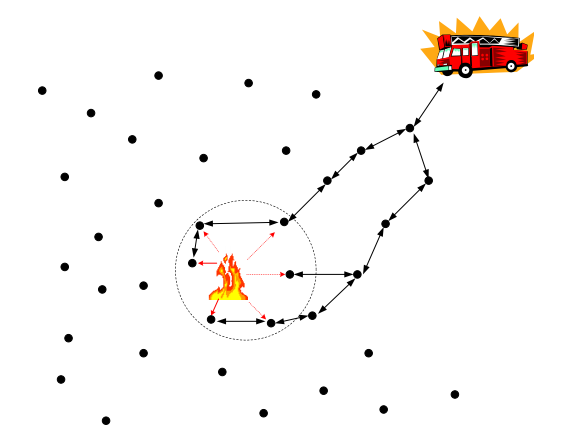
\includegraphics[scale=0.6]{img/lokalisierung_1}

  \caption{Beispiel für die Bedeutung der Lokalisierung in
    Sensornetzen}
  \label{fig:local}
\end{figure}

Abbildung \ref{fig:local} zeigt ein Sensornetz, in dem ein durch einen
Knoten ein Feuer gemeldet wird. Diese Information muss zur Zentrale
weiter geleitet werden, damit dort zum einen die Position des Feuers
bestimmt werden kann. Dafür müssen die Knoten die Position ihrer
Nachbarn kennen und die Position der Basis, damit die Information zum
einen an der richtigen Stelle ankommt. Desweiteren kann so auch der
kürzeste Pfad direkt in der Basis berechnet werden, wenn diese weiß,
wo die Daten herkommen und welche Sensoren sie dafür passiert haben.
\cite{gholami2011} 

Eines der größten Probleme bei der Lokalisierung besteht darin, dass
jedem Knoten nur sehr begreznte Resourcen zur verfügung stehen.
Meistens verfügen diese über einen \ac{uC} der eine geringe
Rechenleistung und Speicherkapazität hat und zudem möglichst
Stromspaarend arbeiten muss. \cite{timmermann} Ein weiteres Problem
besteht darin, dass die Position von Knoten nicht stationär sein muss,
somit müssen die Berechnugen und Messungen direkt von den \ac{uC}'s
durchgeführet und wiederholt werden. \cite{roehrig2009}  Dafür werden
bestimmte Verfahren und Algorithmen benötigt, die wir in dieser
Ausarbeitung vorstellen und diskutieren werden.
\section{Messmethoden}
\subsection{Anchor\/Beacon Nodes}

Als \textit{Anchor- oder Beacon Nodes} werden die Sensorknoten bezeichnet, deren Position in einem globalen Koordinatensystem bekannt sind.
Diese Information kann auf zwei Weisen gewonnen werden. Zum ersten ist es möglich, die Sensorknoten die als Ankerknoten fungieren sollen, 
mit einem GPS-Chip auszustatten und auf diese Weise die Position zu jeder beliebigen Zeit zu ermitteln. Ein solcher Ansatz ist besonders
für den Fall sinnvoll, wenn der Ankerknoten oder sogar das gesammte Sensornetz die Möglichkeit haben soll mobil zu sein. 
Die andere Möglichkeit besteht darin, die exakte Position des Ankerknotens fest einzuprogrammieren. Solch ein Ansatz ist empfehlenswert,
sollte das Sensornetz oder zumindest die Ankerknoten statisch sein. Der große Vorteil dieser Methode der vorprogrammierten Koordinaten ist,
das keinerlei zusätzlich Hardware am Sensorknoten angebracht werden muss und somit keine weiteren finanziellen Kosten anfallen und ebenso der
Energiebedarf der Knoten niedrig gehalten werden kann. \\~\\
Um nun die Ankerknoten effektiv nutzen zu können benötigt man zur Erstellung eines globalen zweidimensionalen Koordinatensystems mindestens
drei Ankerknoten, welche nicht linear angeordnet sein dürfen. Soll sogar ein dreidimensonales globales Koordinatensystem erzeugt werden, wird
ein weitere Ankerknoten benötigt. Hier gilt die Einschränkung des zweidimensionalen Falles und zusätzlich muss der vierte Ankerknoten auf einer
anderen Ebene sein, als die anderen drei. Als sehr effektiv gilt hier die Anordnung als Tetraeder. \\~\\
Um nun unter Zuhilfenahme der Ankerknoten ein Koordinatensystem aufbauen zu können, gibt es zwei Möglichkeiten. Zum einen ist es realisierbar das 
ein mit Hilfe aller Sensorknoten erzeugtes relatives Koordinatensystem, nachträglich auf Ankerknoten gelegt werden und somit die relativen Positionen, 
in globale umrechenbar sind. Andererseits ist es möglich die bekannten Positionen direkt bei den Messungen zu nutzen und so, jede Position eines
Sensorknotens direkt als globale zu errechnen. 

\subsection{Signalstärkemessung}
Die Signalstärkemessung oder \ac{RSSI} basiert auf der Idee, die bei einem kabellosen Sensornetz vorhandenen Sender und Empfänger zu nutzen um die 
Entfernung von Sensorknoten untereinander zu messen. Es wird davon ausgegangen das alle Sensorknoten eine identische Sendeleistung haben und es nun
möglich sein sollte über die ankommende Signalstärke exakt zu berechnen, wie weit der emittierende Sensorknoten vom empfangenden entfernt ist. Als 
physikalische Grundlage dient an dieser Stelle, das die Signalstärke im Vakuum, quadratisch zur zurückgelegten Entfernung abnimmt. In der Praxis 
hat sich allerdings herausgestellt das die Signalstärke durch aller Hand Störfaktoren, wie Luftfeuchtigkeit und -temperatur aber auch Störstrahlung 
und Hindernisse welche das Signal reflektiven oder absorbieren, beeinflusst wird. Die folgende Abbildung zeigt das Ergebnis einer Messreihe und es 
wird hier deutlich, dass das reale Messergebnis in keiner Weise mit dem idealen kreisförmigen Ergebnis der Theorie übereinstimmt. 

\begin{figure}
  \caption{RSSI Meassurement}
  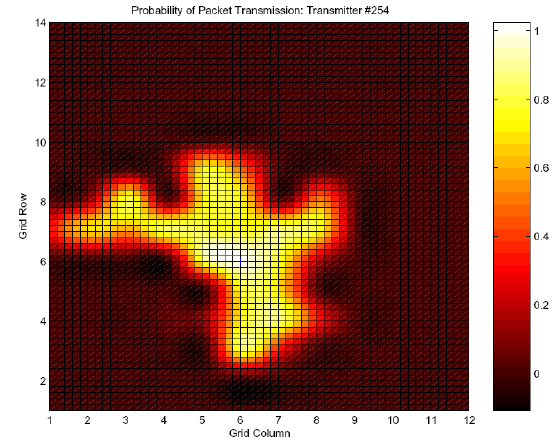
\includegraphics[scale=0.75]{img/RSSI1}\\
  \cite{whitehouse}
\end{figure}

\subsection{Hop Count}
blabla


\section{Algorithmen}
\label{sec:algorithmen}

Zur Auswertung der gesammelten Messaden werden wie in Abbildung
\ref{fig:algo} gezeigt, bestimmte Algorithmen benötigt, um die
Position zu bestimmen. Zwei Grundlegende Methoden zur Bestimmung der
Position sind \textbf{Triangulation} und \textbf{Trilateration}, die
die Grundlage zu anderen Verfahren bilden.

\subsection{Triangulation}

Wird das \ac{AoA} Verfahren verwendet müssen mindestens zwei ortsfeste
Koten $A$ und $B$ so wie die Einfalswinkel $\alpha$ und $\beta$ der
Signale bekannt sein. Dann kann mittels Triangulation (Abbildung
\ref{fig:triang}) die Position eines weiteren Knoten $C$ berechnet
werden. Der Knoten $C$ kann wiederum ein stationärer oder ein mobieler
Knoten sein.

\begin{figure}[h!]
  \centering
  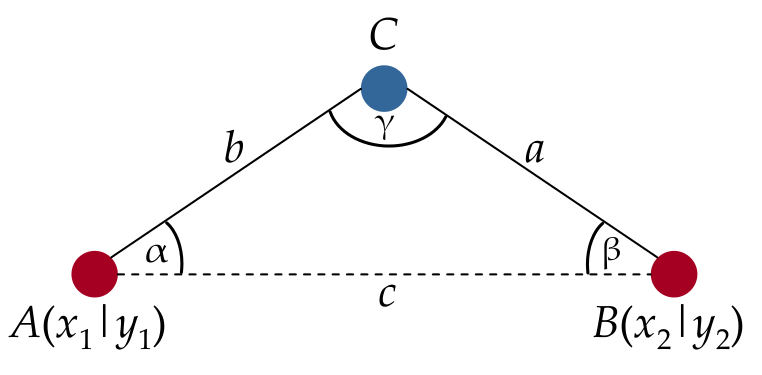
\includegraphics[scale=0.3]{img/triang}

  \caption{Triangulation}
  \label{fig:triang}
\end{figure}

Der Grundgedanke dabei ist, dass theoretisch mit nur zwei bekannten,
ortsfesten Knoten, die Position aller Nachbarn berechnet werden kann.
Sind dabei alle Knoten stationär, ist dies auch möglich, bei mobielen
Knoten kann dies allerdings Problematisch werden, da die Position des
Knotens sich permanent verändern kann. Zudem ist die Genauigkeit der
Triangulation bei mobilen Sensoren sehr schlecht und die Position kann
durch den hohen Messfehler nicht exakt bestimmt werden.
\cite{roehrig2009} 

Die Berechnung mittels Triangulation ist für einen \ac{uC} nicht sehr
aufwendig, da sie nur den Sinus- oder Cosinussatz verwendet. (Gleichung
\ref{eq:triang})

\pagebreak
\begin{framed}
\begin{equation}
  \label{eq:triang}
  c = \sqrt{(B_{x)} - A_{x})^2 + (B_{y} - A_{y})^2}
  ~~~~~~~~
  \varphi = arctan(\frac{B_{y} - A_{y}}{B_{x}} - A_{x})
\end{equation}
\begin{equation*}
  b = c \cdot \frac{sin(\beta)}{sin(\alpha + \beta)}
\end{equation*}
~\\
\begin{equation*}
  C_{x} = A_{x} + b \cdot cos(\varphi)
  ~~~~~~~~
  C_{y} = A_{x} + b \cdot sin(\varphi)
\end{equation*}
\end{framed}
\myequations{Triangulation}


\subsection{Trilateration}

Werden Verfahren wie \ac{ToA}, \ac{TDoA} oder \ac{RToF} eingesetzt,
sind die Winkel der Signale nicht bekannt. Hier werden mindestens
drei ortsfeste Knoten benötigt, um die Position zu einem weiteren
Knoten zu berechnen. Ein weiterer Vorteil der Trilateration ist, dass
die Hardware Anforderungen zur Messung des Einfallwinkels wesentlich
höher sind, als eine reine Distanzmessung. \cite{roehrig2009} 

\begin{figure}[h!]
  \centering
  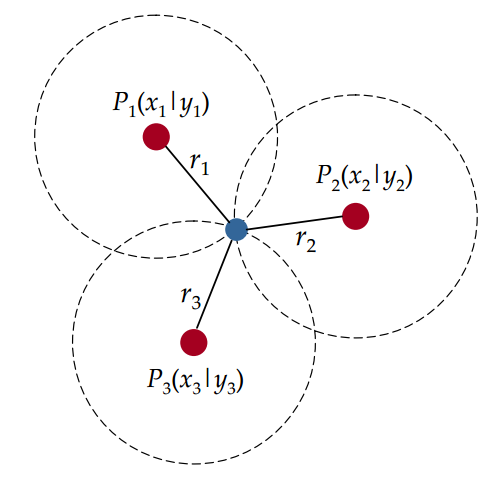
\includegraphics[scale=0.5]{img/trilat}

  \caption{Trilateration}
  \label{fig:trilat}
\end{figure}

Für die Distanz zu den Knoten $P_{¹}$, $P_{2}$ und $P_{3}$ gilt:

\begin{framed}
\begin{equation}
  \label{eq:trilat1}
  r_{i} = \sqrt{(p_{x} - x_{i})^{²} + (p_{y} - y_{i})^{2}}
\end{equation}
\end{framed}
\myequations{Trilateration: Distanz zu stationären Knoten}

Die Position des vierten Knoten lässt sich dann über das
Gleichungssystem \ref{eq:trilat2} berechnen.

\begin{framed}
\begin{equation}
  \label{eq:trilat2}
  \begin{pmatrix}
    P_{x} \\
    P_{y}
  \end{pmatrix}
  =
  H^{-1} \cdot z
\end{equation}
\begin{equation*}
  H = 
  \begin{bmatrix}
    2 \cdot x_{1} - 2 \cdot x_{2} & 2 \cdot y_{1} - 2 \cdot y_{2} \\
    2 \cdot x_{1} - 2 \cdot x_{3} & 2 \cdot y_{1} - 2 \cdot y_{3}
  \end{bmatrix}
\end{equation*}
\begin{equation*}
  z = 
  \begin{pmatrix}
    r_{2}^2 - r_{1}^2 + x_{1}^2 - x_{2}^2 + y_{1}^2 - y_{2}^2 \\
    r_{3}^2 - r_{1}^2 + x_{1}^2 - x_{3}^2 + y_{1}^2 - y_{3}^2
  \end{pmatrix}
\end{equation*}
\end{framed}
\myequations{Trilateration: Gleichungssystem}


\subsection{Weiterführende Algorithmen}

Wie bereits beschrieben, bieten die beiden geziegten Verfahren nur
ungenaue Ergebnisse, vor allem bei mobielen Knoten ist der Fehler sehr
groß. Auß diesem Grund werden weitere Verfahren benötigt, um die
Wahrscheinlichkeit zu maximieren, dass die berechnete Position stimmt.

% TODO Algos hinzufügen 

\newpage
\pagenumbering{roman}
\addcontentsline{toc}{section}{Literatur}
\bibliographystyle{agsm}
\bibliography{references}
\end{document}
